% \begin{figure}[htbp]
%     \centering
%     \vspace{-8px}
%     \includegraphics[width=0.8\linewidth]{figures/teaser.pdf}
%     \vspace{-5px}
%     \caption{\textbf{Performance and prompt stability analysis across different prompt optimization methods.} 
%     We evaluate baseline and other prompt optimization methods, measuring average win-rate and normalized standard deviation. 
%     Result demonstrates that our method COPER delivers higher win-rates than all alternatives and also exhibits greater stability.}
%     \label{fig:teaser}
% \end{figure}


% \begin{figure*}[h!]
%     \centering
%     \vspace{-10px}
%     \begin{subfigure}[b]{0.48\linewidth}
%         \centering
%         \includegraphics[width=\linewidth, height=5.4cm, keepaspectratio=false]{figures/teaser.pdf}
%         \caption{\textbf{Performance and prompt stability analysis across different prompt optimization methods.}}
%         \label{fig:teaser_a}
%     \end{subfigure}
%     \vspace{-3px}
%     \hfill
%     \begin{subfigure}[b]{0.48\linewidth}
%         \centering
%         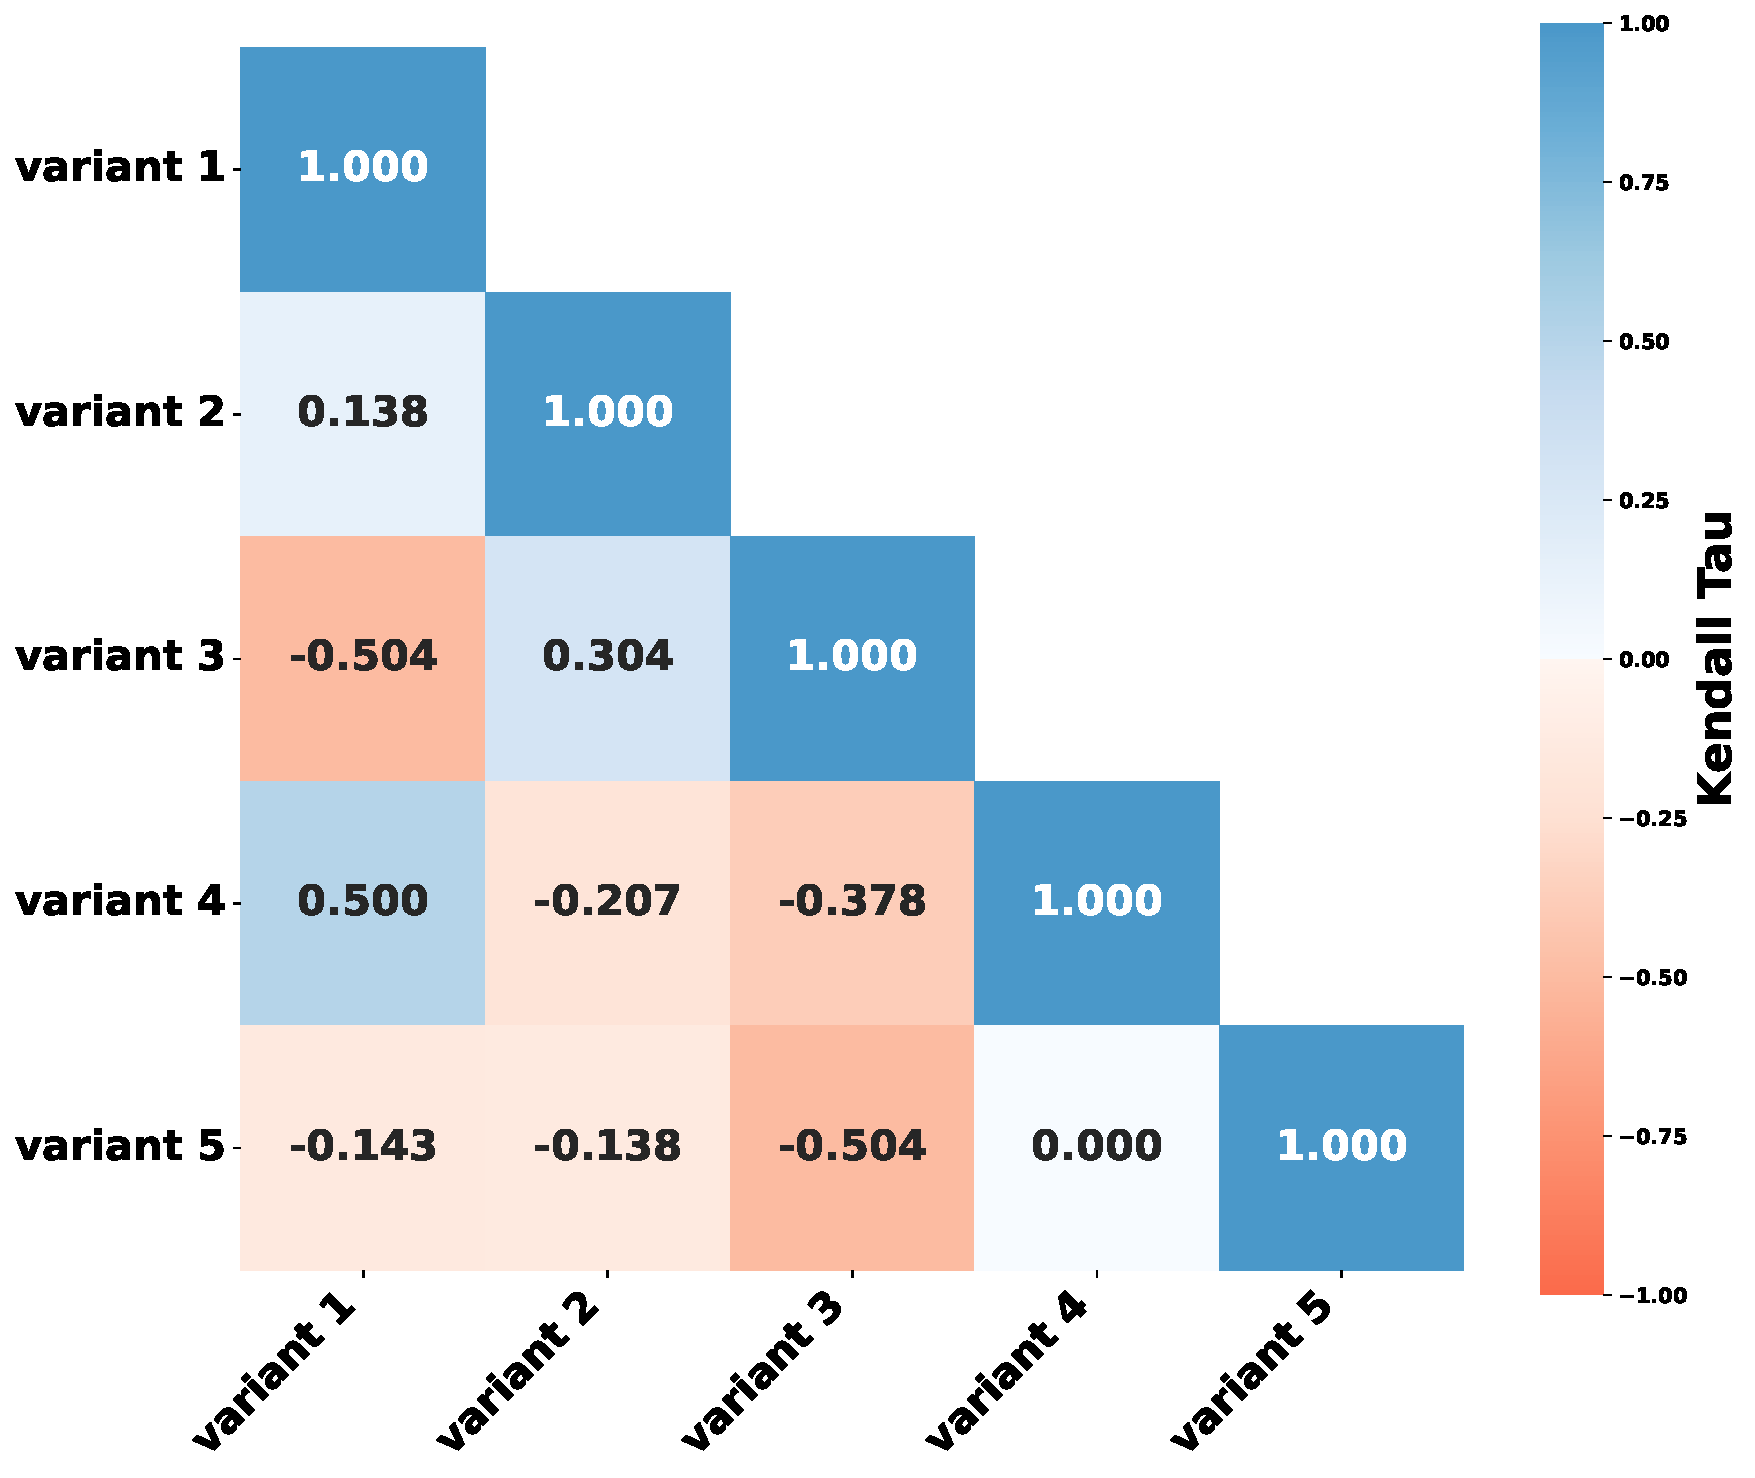
\includegraphics[width=\linewidth, height=5.4cm, keepaspectratio=false]{figures/kendall_tau.pdf}
% \caption{\textcolor{red}{This would be replaced by an trian effiency graph later, and this current graph would be moved tothe  appendix}\textbf{Ranking sensitivity in \textsc{KuhnPoker}.} }
%         \label{fig:teaser_b}
%     \end{subfigure}
%     \vspace{-3px}
%     \label{fig:teaser}
%     \caption{\textbf{Left:} We evaluate baseline and other prompt optimization methods by average win-rate and RSE. Our method, COPER, achieved the highest win-rates and the lowest variance, demonstrating enhanced performance and stability. \textbf{Right:} With environment and evaluator pools fixed, five \emph{nearly equivalent} prompt variants still flip pairwise outcomes and reshuffle rankings (detailed prompt variants are presented in Appendix~\ref{appendix:prompt_variants}). The heatmap shows Kendall's $\tau_b$ for every pair of prompts: blue means very similar rankings ($\tau_b \approx 1$), white means unstable rankings ($\tau_b \approx 0$), and orange means rank reversals ($\tau_b < 0$).}
% \end{figure*}

\begin{figure}[H]
    \centering
    \vspace{-3px}
    \begin{subfigure}[b]{0.49\linewidth}
        \centering
        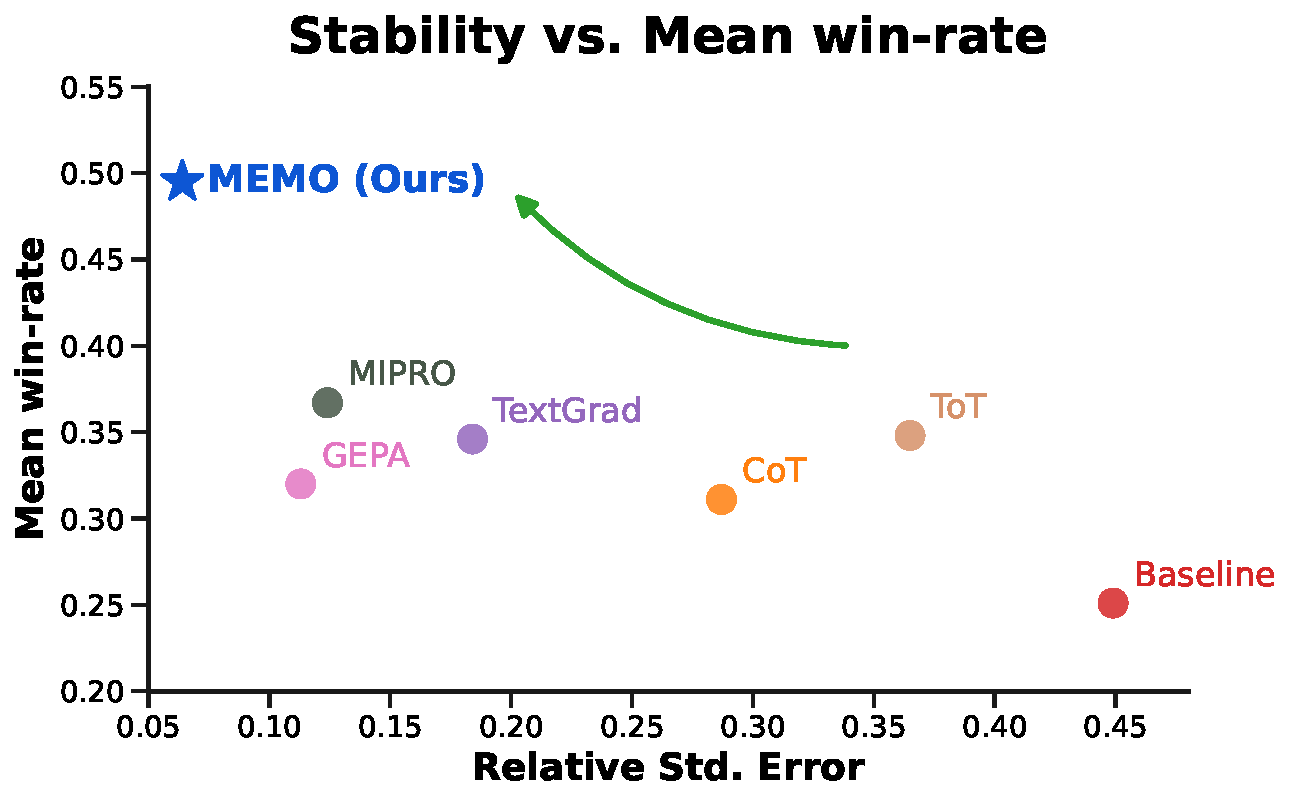
\includegraphics[width=.95\linewidth, keepaspectratio=false]{figures/teaser_bar.pdf}
        \caption{\textbf{Performance and stability across methods.}}
        \label{fig:teaser_a}
    \end{subfigure}
    \vspace{-3px}
    \hfill
    \begin{subfigure}[b]{0.48\linewidth}
        \centering
        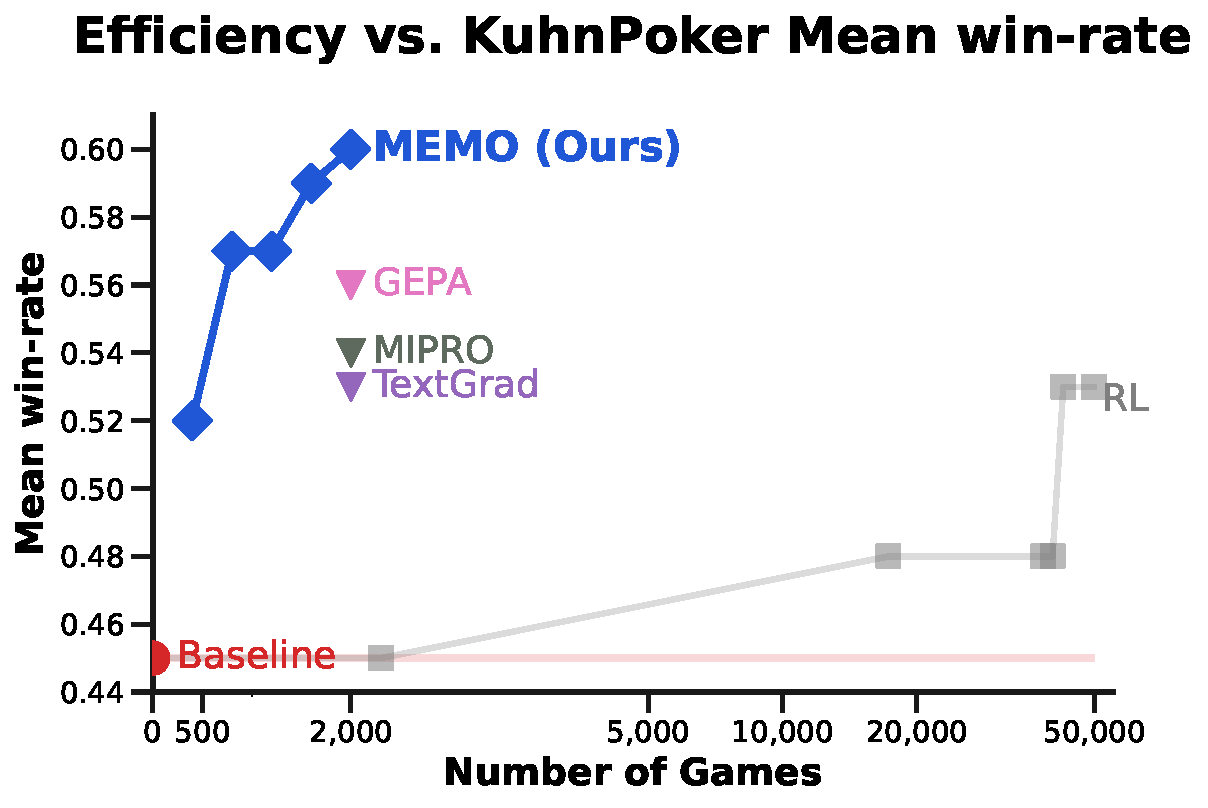
\includegraphics[width=.9\linewidth, keepaspectratio=false]{figures/kuhnpoker_winrate_style.pdf}
        \caption{\textbf{Training Efficiencies in \textsc{KuhnPoker}.}}
        \label{fig:teaser_b}
    \end{subfigure}
    \vspace{-3px}
    \label{fig:teaser}
\caption{\textbf{Left} Run-to-run performance and stability comparison. Using GPT-4o-mini with \NAME{} achieves the highest mean win rate (49.5\%) with the lowest RSE (6.4\%). \textbf{Right} Learning efficiency comparison against the self-play RL baseline method \textsc{Unstablebaseline}. Using Qwen2.5-7B-Instruct, \NAME{} reaches 60\% win rate on Kuhn Poker with only 2{,}000 games, 19$\times$ fewer than the 38{,}000 games required by the RL self-play baseline.}
    % \textcolor{red}{updating the figures, and would update caption afterward}
\end{figure}

% \caption{\textbf{Right:} Win rate as a function of environment interactions (games played), measuring sample efficiency. \NAME{} reaches the top win rate using the fewest games among all methods.}
% \caption{\textbf{Left:} Mean win rate versus relative standard error (RSE) for the baseline and prompt-optimization baselines. \NAME{} achieves the highest mean win rate (49.5\%) with the lowest RSE (6.4\%). \textbf{Right:} Learning curves comparing our self-play \NAME{} context optimization method with the self-play RL baseline (\textsc{Unstablebaseline}). \NAME{} reaches 60\% win rate using 2{,}000 games.}
